%%%%%%%%%%%%  Generated using docx2latex.com  %%%%%%%%%%%%%%

%%%%%%%%%%%%  v2.0.0-beta  %%%%%%%%%%%%%%

\documentclass[12pt]{article}
\usepackage{amsmath}
\usepackage{latexsym}
\usepackage{amsfonts}
\usepackage[normalem]{ulem}
\usepackage{array}
\usepackage{amssymb}
\usepackage{graphicx}
\usepackage{subfig}
\usepackage{wrapfig}
\usepackage{wasysym}
\usepackage{enumitem}
\usepackage{adjustbox}
\usepackage{ragged2e}
\usepackage[svgnames,table]{xcolor}
\usepackage{tikz}
\usepackage{longtable}
\usepackage{changepage}
\usepackage{setspace}
\usepackage{hhline}
\usepackage{multicol}
\usepackage{tabto}
\usepackage{float}
\usepackage{multirow}
\usepackage{makecell}
\usepackage{fancyhdr}
\usepackage[toc,page]{appendix}
\usepackage[paperheight=11.69in,paperwidth=8.27in,left=1.18in,right=1.18in,top=1.38in,bottom=0.98in,headheight=1in]{geometry}
\usepackage[utf8]{inputenc}
\usepackage[T1]{fontenc}
\usepackage[hidelinks]{hyperref}
\usetikzlibrary{shapes.symbols,shapes.geometric,shadows,arrows.meta}
\tikzset{>={Latex[width=1.5mm,length=2mm]}}
\usepackage{flowchart}\TabPositions{0.5in,1.0in,1.5in,2.0in,2.5in,3.0in,3.5in,4.0in,4.5in,5.0in,5.5in,}

\urlstyle{same}


 %%%%%%%%%%%%  Set Depths for Sections  %%%%%%%%%%%%%%

% 1) Section
% 1.1) SubSection
% 1.1.1) SubSubSection
% 1.1.1.1) Paragraph
% 1.1.1.1.1) Subparagraph


\setcounter{tocdepth}{5}
\setcounter{secnumdepth}{5}


 %%%%%%%%%%%%  Set Depths for Nested Lists created by \begin{enumerate}  %%%%%%%%%%%%%%


\setlistdepth{9}
\renewlist{enumerate}{enumerate}{9}
	\setlist[enumerate,1]{label=\arabic*)}
	\setlist[enumerate,2]{label=\alph*)}
	\setlist[enumerate,3]{label=(\roman*)}
	\setlist[enumerate,4]{label=(\arabic*)}
	\setlist[enumerate,5]{label=(\Alph*)}
	\setlist[enumerate,6]{label=(\Roman*)}
	\setlist[enumerate,7]{label=\arabic*}
	\setlist[enumerate,8]{label=\alph*}
	\setlist[enumerate,9]{label=\roman*}

\renewlist{itemize}{itemize}{9}
	\setlist[itemize]{label=$\cdot$}
	\setlist[itemize,1]{label=\textbullet}
	\setlist[itemize,2]{label=$\circ$}
	\setlist[itemize,3]{label=$\ast$}
	\setlist[itemize,4]{label=$\dagger$}
	\setlist[itemize,5]{label=$\triangleright$}
	\setlist[itemize,6]{label=$\bigstar$}
	\setlist[itemize,7]{label=$\blacklozenge$}
	\setlist[itemize,8]{label=$\prime$}



 %%%%%%%%%%%%  Header here  %%%%%%%%%%%%%%


\pagestyle{fancy}
\fancyhf{}
\chead{ }
\cfoot{ 
\vspace{\baselineskip}
}
\renewcommand{\headrulewidth}{0pt}
\setlength{\topsep}{0pt}\setlength{\parindent}{0pt}
\renewcommand{\arraystretch}{1.3}


%%%%%%%%%%%%%%%%%%%% Document code starts here %%%%%%%%%%%%%%%%%%%%



\begin{document}
\begin{Center}
{\fontsize{16pt}{19.2pt}\selectfont \textbf{Título do Trabalho}\par}
\end{Center}\par

\begin{Center}
{\fontsize{11pt}{13.2pt}\selectfont Trabalho de Conclusão do Curso de\par}
\end{Center}\par

\begin{Center}
{\fontsize{11pt}{13.2pt}\selectfont Tecnologia em Sistemas Para Internet\par}
\end{Center}\par

\begin{Center}
\textbf{Nome do Aluno}
\end{Center}\par

\begin{Center}
{\fontsize{11pt}{13.2pt}\selectfont Orientador(a): Fulano de Tal\par}
\end{Center}\par

\begin{Center}
\textsuperscript{1}Instituto Federal de Educação, Ciência e Tecnologia do Rio Grande do Sul (IFRS)\\
Campus Porto Alegre\\
Av Cel Vicente, 281, Porto Alegre – RS – Brasil
\end{Center}\par

\begin{Center}
{\fontsize{10pt}{12.0pt}\selectfont aluno@gmail.com, prof@poa.ifrs.edu.br\par}
\end{Center}\par

\textit{\textbf{Resumo. Este meta-artigo descreve o estilo a ser usado na confecção de artigos e resumos de artigos para publicação nos anais das conferências organizadas pela SBC. É solicitada a escrita de resumo e abstract apenas para os artigos escritos em português. Artigos em inglês deverão apresentar apenas abstract. Nos dois casos, o autor deve tomar cuidado para que o resumo (e o abstract) não ultrapassem 10 linhas cada, sendo que ambos devem estar na primeira página do artigo.}}\par

\section*{1. General Information}
\addcontentsline{toc}{section}{1. General Information}
All full papers and posters (short papers) submitted to some SBC conference, including any supporting documents, should be written in English or in Portuguese. The format paper should be A4 with single column, 3.5 cm for upper margin, 2.5 cm for bottom margin and 3.0 cm for lateral margins, without headers or footers. The main font must be Times, 12 point nominal size, with 6 points of space before each paragraph. Page numbers must be suppressed. \par

\tab Full papers must respect the page limits defined by the conference. Conferences that publish just abstracts ask for \textbf{one}-page texts.\par

\section*{2. First Page}
\addcontentsline{toc}{section}{2. First Page}
The first page must display the paper title, the name and address of the authors, the abstract in English and $``$resumo$"$  in Portuguese ($``$resumos$"$  are required only for papers written in Portuguese). The title must be centered over the whole page, in 16 point boldface font and with 12 points of space before itself. Author names must be centered in 12 point font, bold, all of them disposed in the same line, separated by commas and with 12 points of space after the title. Addresses must be centered in 12 point font, also with 12 points of space after the authors’ names. E-mail addresses should be written using font Courier New, 10 point nominal size, with 6 points of space before and 6 points of space after.\par

\tab The abstract and $``$resumo$"$  (if is the case) must be in 12 point Times font, indented 0.8cm on both sides. The word \textbf{Abstract }and \textbf{Resumo}, should be written in boldface and must precede the text.\par

\section*{3. CD-ROMs and Printed Proceedings}
\addcontentsline{toc}{section}{3. CD-ROMs and Printed Proceedings}
In some conferences, the papers are published on CD-ROM while only the abstract is published in the printed Proceedings. In this case, authors are invited to prepare two final versions of the paper. One,\ complete, to be published on the CD and the other, containing only the first page, with abstract and $``$resumo$"$  (for papers in Portuguese).  \par

\section*{4. Sections and Paragraphs}
\addcontentsline{toc}{section}{4. Sections and Paragraphs}
Section titles must be in boldface, 13pt, flush left. There should be an extra 12 pt of space before each title. Section numbering is optional. The first paragraph of each section should not be indented, while the first lines of subsequent paragraphs should be indented by 1.27 cm. \par

\subsection*{4.1. Subsections}
\addcontentsline{toc}{subsection}{4.1. Subsections}
The subsection titles must be in boldface, 12pt, flush left.\par

\section*{5. Figures and Captions}
\addcontentsline{toc}{section}{5. Figures and Captions}
Figure and table captions should be centered if less than one line (Figure 1), otherwise justified and indented by 0.8cm on both margins, as shown in Figure 2. The caption font must be Helvetica, 10 point, boldface, with 6 points of space before and after each caption. \par



%%%%%%%%%%%%%%%%%%%% Figure/Image No: 1 starts here %%%%%%%%%%%%%%%%%%%%

\begin{figure}[H]
	\begin{Center}
		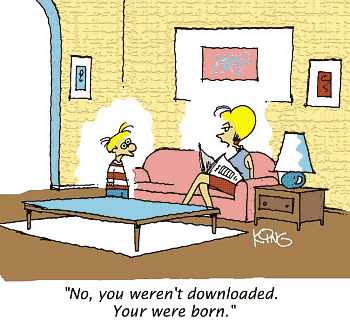
\includegraphics[width=245.25pt,height=223.5pt]{./media/image1.png}
		\caption{. A typical figure}
		\label{fig:. A typical figure}
	\end{Center}
\end{figure}


%%%%%%%%%%%%%%%%%%%% Figure/Image No: 1 Ends here %%%%%%%%%%%%%%%%%%%%


\vspace{\baselineskip}
\par



%%%%%%%%%%%%%%%%%%%% Figure/Image No: 2 starts here %%%%%%%%%%%%%%%%%%%%

\begin{figure}[H]
	\begin{Center}
		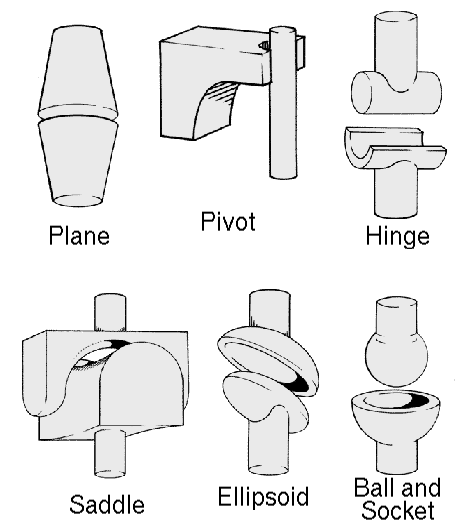
\includegraphics[width=195.75pt,height=219.75pt]{./media/image2.png}
		\caption{. This figure is an example of a figure caption taking more than one line and justified considering margins mentioned in Section 5.}
		\label{fig:. This figure is an example of a figure caption taking more than one line and justified considering margins mentioned in Section 5.}
	\end{Center}
\end{figure}


%%%%%%%%%%%%%%%%%%%% Figure/Image No: 2 Ends here %%%%%%%%%%%%%%%%%%%%


\vspace{\baselineskip}
\par

\tab In tables, try to avoid the use of colored or shaded backgrounds, and avoid thick, doubled, or unnecessary framing lines. When reporting empirical data, do not use more decimal digits than warranted by their precision and reproducibility. Table caption must be placed before the table (see Table 1) and the font used must also be Helvetica, 10 point, boldface, with 6 points of space before and after each caption.\par

\par



%%%%%%%%%%%%%%%%%%%% Figure/Image No: 3 starts here %%%%%%%%%%%%%%%%%%%%

\begin{figure}[H]
	\begin{Center}
		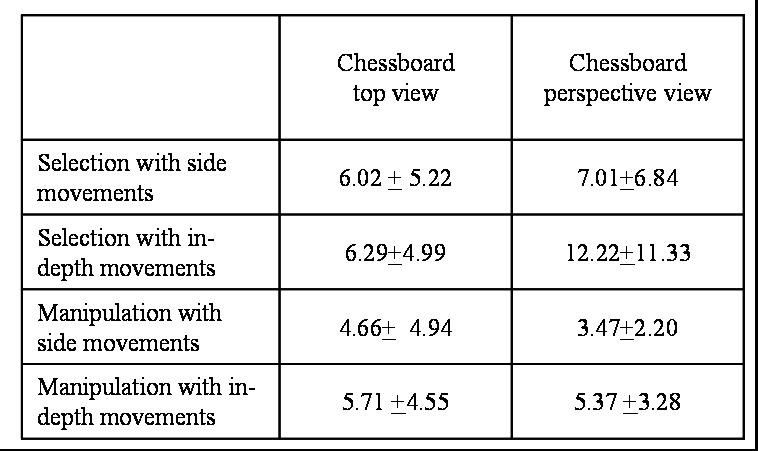
\includegraphics[width=309pt,height=183pt]{./media/image3.jpeg}
	\end{Center}
\end{figure}


%%%%%%%%%%%%%%%%%%%% Figure/Image No: 3 Ends here %%%%%%%%%%%%%%%%%%%%


\vspace{\baselineskip}
\section*{6. Images}
\addcontentsline{toc}{section}{6. Images}
All images and illustrations should be in black-and-white, or gray tones, excepting for the papers that will be electronically available (on CD-ROMs, internet, etc.). The image resolution on paper should be about 600 dpi for black-and-white images, and 150-300 dpi\ for grayscale images.  Do not include images with excessive resolution, as they may take hours to print, without any visible difference in the result.\par

\par

Bibliographic\ references must be unambiguous and uniform.  We recommend giving the author names references in brackets, e.g. [Knuth 1984], [Boulic and Renault 1991]; or dates in parentheses, e.g. Knuth (1984), Smith and Jones (1999).\par

\tab The references must be listed using 12 point font size, with 6 points of space before each reference. The first line of each reference should not be indented, while the subsequent should be indented by 0.5 cm.\par

\par

Boulic, R. and Renault, O. (1991) $``$3D Hierarchies for Animation$"$ , In: New Trends in Animation and Visualization, Edited by Nadia Magnenat-Thalmann and Daniel Thalmann, John Wiley $\&$  Sons ltd., England.\par

Dyer, S., Martin, J. and Zulauf, J. (1995) $``$Motion Capture White Paper$"$ , \href{http://reality.sgi.com/employees/jam\_sb/mocap/MoCapWP\_v2.0.html}{http://reality.sgi.com/employees/jam\_sb/mocap/MoCapWP\_v2.0.html}, December.\par

Holton, M. and Alexander, S. (1995) $``$Soft Cellular Modeling: A Technique for the Simulation of Non-rigid Materials$"$ , Computer Graphics: Developments in Virtual Environments, R. A. Earnshaw and J. A. Vince, England, Academic Press Ltd., p. 449-460.\par

Knuth, D. E. (1984), The TeXbook, Addison Wesley, 15\textsuperscript{th} edition. \par

Smith, A. and Jones, B. (1999). On the complexity of computing. In \textit{Advances in Computer Science}, pages 555–566. Publishing Press.\par


\vspace{\baselineskip}

\vspace{\baselineskip}
\end{document}